\section{Experimental results}
\label{sec:results}

Experimental data were collected using three machines:
\begin{itemize}
    \item \textbf{Machine A}: \textbf{Intel Core i7-8750H} (8th gen, 6 cores, 12 threads, up to 4{,}1~GHz), \textbf{16~GB DDR4 RAM}, SSD \textbf{SanDisk 128~GB SATA M.2} (\texttt{SD9SN8W128G1002}), operating system \textbf{Arch Linux}, kernel \texttt{6.15.6}, file system \texttt{btrfs}.
    \item \textbf{Machine B}: \textbf{Intel Core i7-12700H} (12th gen, 14 cores, 20 threads, up to 4{,}7~GHz), \textbf{16~GB DDR4 RAM}, \textbf{1~TB NVMe PCIe} SSD (\texttt{MTFDKBA1T0TFH-1BC1AABHA}), operating system \textbf{Ubuntu 22.04}, kernel \texttt{6.12.10}, file system \texttt{ext4}.
    \item \textbf{Machine C}: \textbf{Intel Core i5-12450H} (12th gen, 8 cores, 12 threads, up to 4{,}4~GHz), \textbf{16~GB DDR4 RAM}, \textbf{512~GB NVMe PCIe} SSD (generic model \texttt{PCIe-8 SSD 512GB}), operating system \textbf{Arch Linux}, kernel \texttt{6.15.6}, file system \texttt{xfs}.
\end{itemize}

The machines were connected via a gigabit Ethernet network with a latency of about 0{,}3~ms.
They were configured with frequency scaling, turbo boost, and hyper-threading disabled to ensure consistent performance and reduce result variability.

The graphs show the observed latency as the operation frequency varies, for different percentiles (from P0 to P100).
Each test was run for a period of 20~seconds, with a frequency increasing from 1000~Hz until the system failed.

\subsection{\texttt{set} operation}
\label{subsec:set-operation}

\begin{figure}[htbp]
    \centering
    \begin{minipage}[t]{0.48\textwidth}
        \centering
        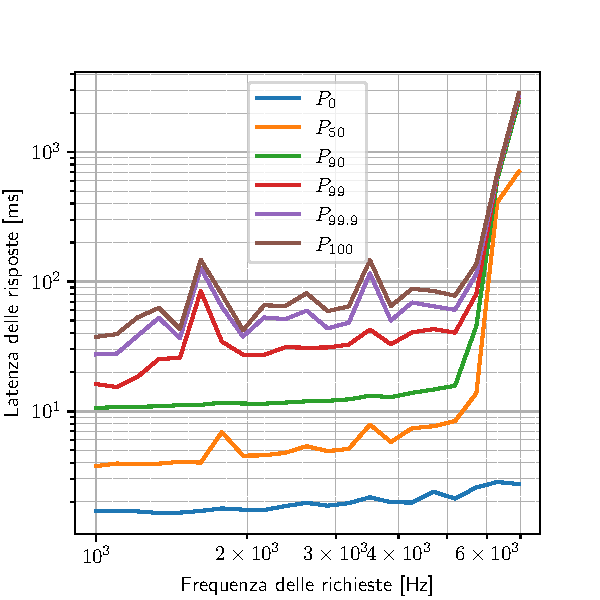
\includegraphics[width=\textwidth]{03-results/bench-set-a}
        \caption*{Machine A}
    \end{minipage}
    \hfill
    \begin{minipage}[t]{0.48\textwidth}
        \centering
        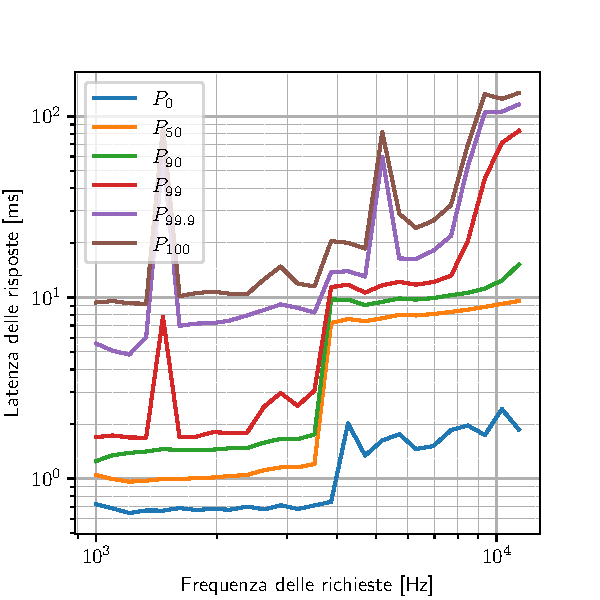
\includegraphics[width=\textwidth]{03-results/bench-set-c}
        \caption*{Machine B}
    \end{minipage}

    \vspace{0.5cm}
    \begin{minipage}[t]{0.48\textwidth}
        \centering
        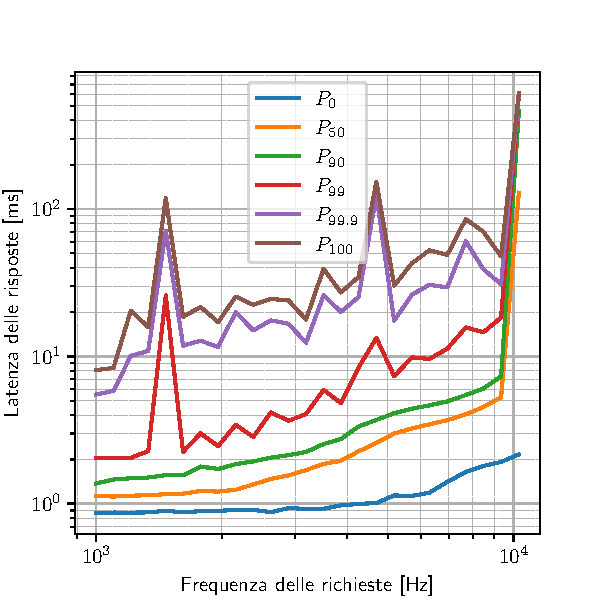
\includegraphics[width=\textwidth]{03-results/bench-set-h}
        \caption*{Machine C}
    \end{minipage}

    \caption{Write performance of the machines. Each graph shows, as the operation frequency [Hz] varies, the observed latency [ms] for different percentiles (from P0 to P100).}
    \label{fig:bench-set}
\end{figure}

\begin{figure}[htbp]
    \centering
    \begin{minipage}[t]{0.48\textwidth}
        \centering
        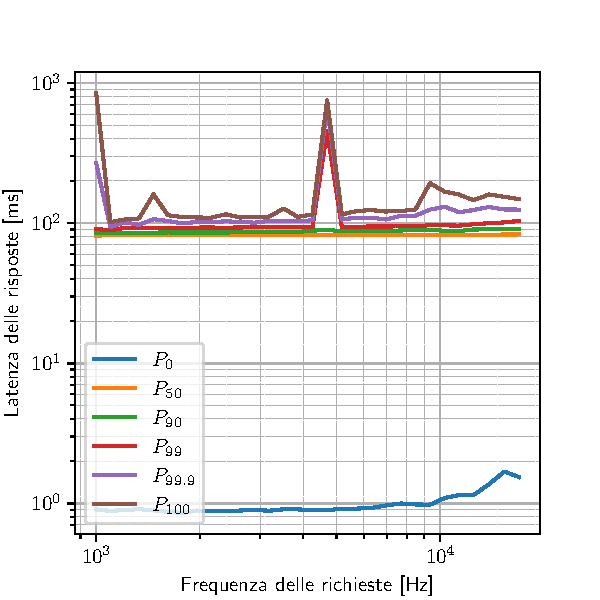
\includegraphics[width=\textwidth]{03-results/bench-set-all}
        \caption*{Keys uniformly distributed across the three machines}
    \end{minipage}
    \hfill
    \begin{minipage}[t]{0.48\textwidth}
        \centering
        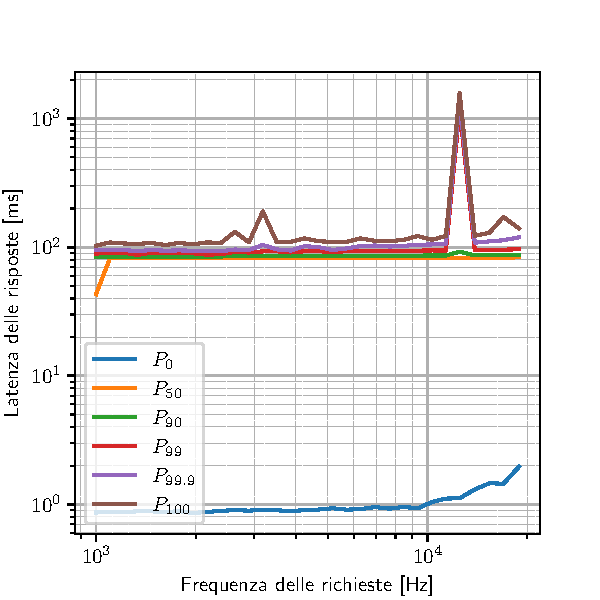
\includegraphics[width=\textwidth]{03-results/bench-set-all-balance}
        \caption*{Keys distributed across the three machines with balanced weights $6{:}10{:}10$}
    \end{minipage}

    \caption{Write performance with distributed keys. Each graph shows, as the operation frequency [Hz] varies, the observed latency [ms] for different percentiles (from P0 to P100).}
    \label{fig:bench-set-all}
\end{figure}

Figure~\ref{fig:bench-set} shows the results obtained by the three machines during write (\texttt{set}) operations.
During the tests, throughput throttling was disabled, allowing the maximum performance of each machine to be observed.
The graphs show that machines A, B, and C reached maximum throughputs of $6{,}9\,{\times}\,10^3$, $11{,}3\,{\times}\,10^3$, and $10{,}3\,{\times}\,10^3$ operations per second, respectively.

Figure~\ref{fig:bench-set-all} presents the results obtained by using the three machines together, with keys distributed among them without replication (parameters $n=1, r=1, w=1$).
When keys were distributed uniformly (with all $b_i$ equal), a total throughput of $16{,}9\,{\times}\,10^3$ operations per second was achieved.
Using a weighted distribution of keys with weights $6{:}10{:}10$, the total throughput rose to $18{,}8\,{\times}\,10^3$ operations per second, demonstrating the importance of the bandwidth allocation mechanism for optimizing performance in heterogeneous scenarios.
Although the sum of the individual capacities is $28{,}6\,{\times}\,10^3$ operations per second, the observed value is lower.
An increase in latency compared to running on a single machine is also observed; however, unlike the single-machine tests, latency remains roughly constant as the operation frequency increases.
These effects are hypothesized to stem from the overhead introduced by communication and coordination among distributed nodes.

\subsection{\texttt{get} operation}
\label{subsec:get-operation}

\begin{figure}[htbp]
    \centering
    \begin{minipage}[t]{0.48\textwidth}
        \centering
        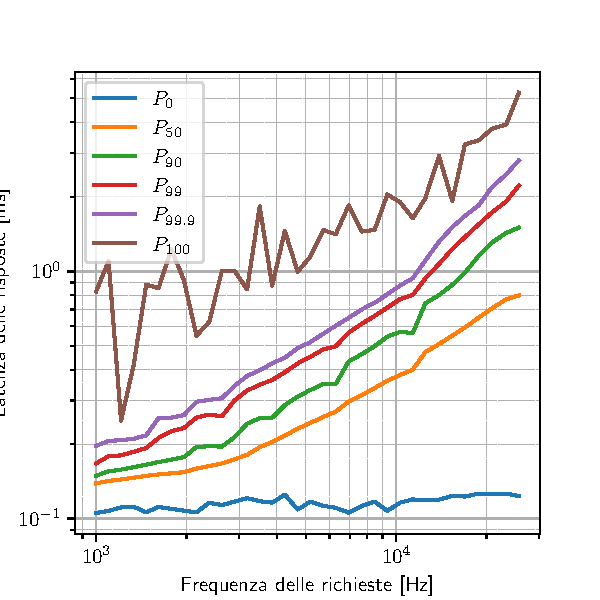
\includegraphics[width=\textwidth]{03-results/bench-get-a}
        \caption*{Machine A}
    \end{minipage}
    \hfill
    \begin{minipage}[t]{0.48\textwidth}
        \centering
        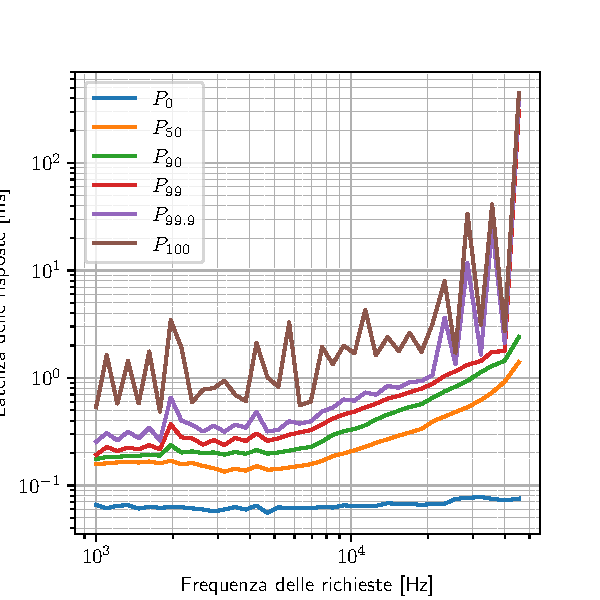
\includegraphics[width=\textwidth]{03-results/bench-get-c}
        \caption*{Machine B}
    \end{minipage}

    \vspace{0.5cm}
    \begin{minipage}[t]{0.48\textwidth}
        \centering
        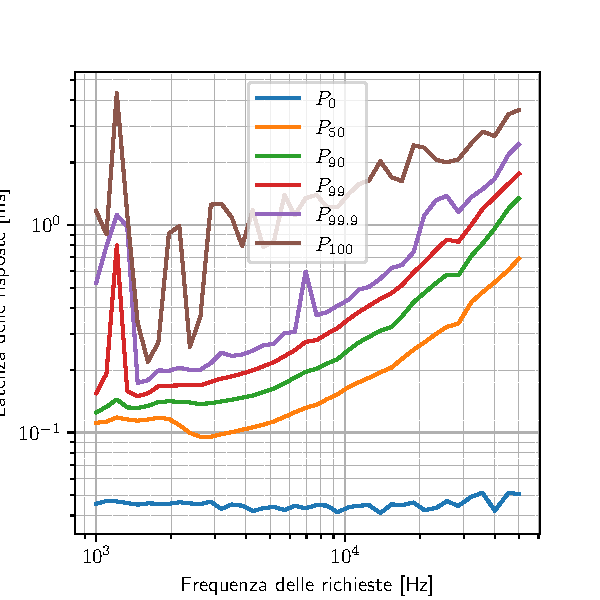
\includegraphics[width=\textwidth]{03-results/bench-get-h}
        \caption*{Machine C}
    \end{minipage}
    \hfill
    \begin{minipage}[t]{0.48\textwidth}
        \centering
        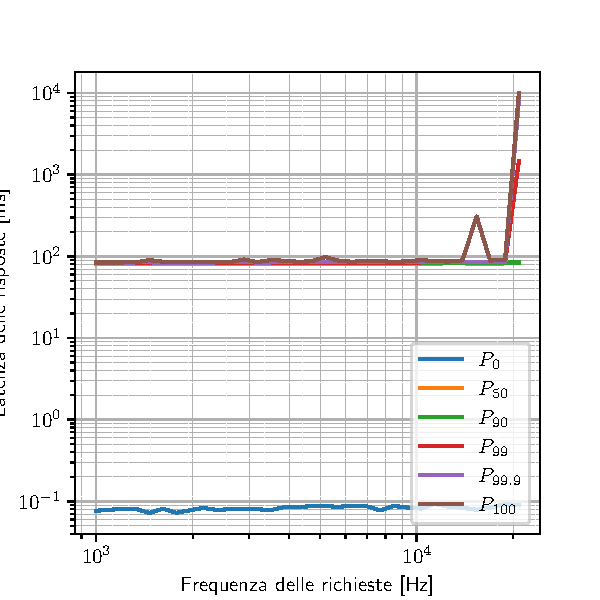
\includegraphics[width=\textwidth]{03-results/bench-get-all}
        \caption*{Keys uniformly distributed across the three machines}
    \end{minipage}

    \caption{Read performance of the machines. Each graph shows, as the operation frequency [Hz] varies, the observed latency [ms] for different percentiles (from P0 to P100).}
    \label{fig:bench-get}
\end{figure}

Figure~\ref{fig:bench-get} shows the results obtained by the three machines during read (\texttt{get}) operations.
Again, throughput throttling was disabled to observe maximum performance.
Machines A, B, and C reached maximum throughputs of $25{,}6\,{\times}\,10^3$, $45{,}4\,{\times}\,10^3$, and $50{,}0\,{\times}\,10^3$ operations per second, respectively.

Using the three machines together with keys uniformly distributed among them and without replication ($n=1, r=1, w=1$), a total throughput of $20{,}8\,{\times}\,10^3$ operations per second was achieved, lower than that of the individual machines.
The cost of a disk read is much lower than that of a write thanks to the file system cache.
This highlights the overhead of communication between machines, which negatively affects overall performance.
It is hypothesized that using a database larger than the available RAM (thereby reducing cache effectiveness) could make multi-machine usage advantageous again.
However, this hypothesis could not be directly verified.

\subsection{Multitenant}
\label{subsec:multitenant}

\begin{figure}[htbp]
    \centering
    \begin{minipage}[t]{0.48\textwidth}
        \centering
        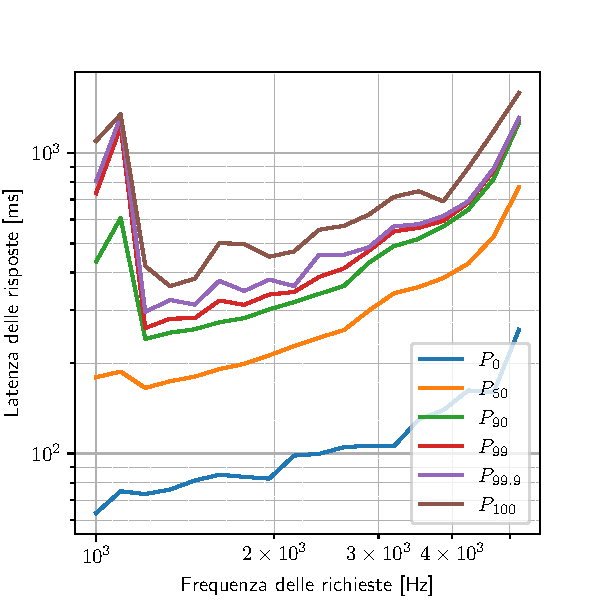
\includegraphics[width=\textwidth]{03-results/bench-set-no-throttling}
        \caption*{Without throughput throttling}
    \end{minipage}
    \hfill
    \begin{minipage}[t]{0.48\textwidth}
        \centering
        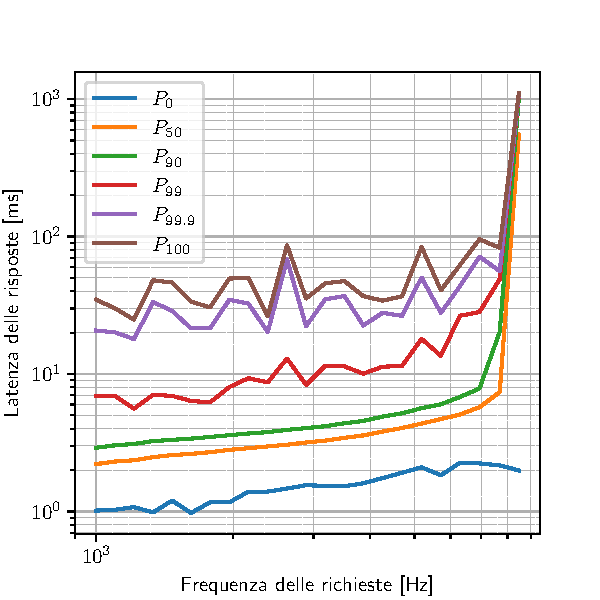
\includegraphics[width=\textwidth]{03-results/bench-set-throttling}
        \caption*{With throughput throttling}
    \end{minipage}

    \caption{Write performance of the machine with and without throughput throttling in the presence of malicious clients. Each graph shows, as the operation frequency [Hz] varies, the observed latency [ms] for different percentiles (from P0 to P100).}
    \label{fig:bench-throttling}
\end{figure}

Figure~\ref{fig:bench-throttling} reports the results obtained by machine C during write operations in a multitenant context.
During the test two tables, X and Y, were present, with bandwidths of 8000 and 1000 operations per second, and a malicious client attempting to saturate resources by writing to table Y.
The malicious client consisted of two parts:
\begin{itemize}
    \item A component that launches 1000 tasks, each performing continuous writes to table Y, thus keeping 1000 concurrent operations always in progress.
    \item A component that generates 4000 operations per second asynchronously, waiting in the background for each request to complete without blocking the main thread.
\end{itemize}

The graphs show the observed performance for table X, with and without throughput throttling (see Section~\ref{subsec:throughput-throttling}).
Without throttling, the latency at the $50^\text{th}$ percentile starts around 180~ms and the maximum throughput reached is $5{,}2\,{\times}\,10^3$ operations per second, lower than the guaranteed value.
With throttling enabled, instead, the latency at the $50^\text{th}$ percentile remains below 10~ms until the guaranteed maximum throughput of 8000 operations per second is reached.
